% Created 2022-03-04 Fri 20:57
% Intended LaTeX compiler: pdflatex
\documentclass[11pt]{article}
\usepackage[utf8]{inputenc}
\usepackage[T1]{fontenc}
\usepackage{graphicx}
\usepackage{grffile}
\usepackage{longtable}
\usepackage{wrapfig}
\usepackage{rotating}
\usepackage[normalem]{ulem}
\usepackage{amsmath}
\usepackage{textcomp}
\usepackage{amssymb}
\usepackage{capt-of}
\usepackage{hyperref}
\author{190022658}
\date{\today}
\title{Report}
\hypersetup{
 pdfauthor={190022658},
 pdftitle={Report},
 pdfkeywords={},
 pdfsubject={},
 pdfcreator={Emacs 27.2 (Org mode 9.5)}, 
 pdflang={English}}
\begin{document}

\maketitle

\section{Overview}
\label{sec:org38a2d65}
In the practical we were given a scenario and were required to design an ER model for it. We then needed to convert the model into a relational schema and identify all the full functional dependencies in the relational schema. Using that we needed to show which normalisation form was achieved.\\

All of the listed requirements have been done.
\section{ER Diagram}
\label{sec:org5ced7e5}
The ER diagram is in the same folder in two formats, it can be opened in the browser in the svg format and in diagrams.net in the drawio format.
\begin{center}
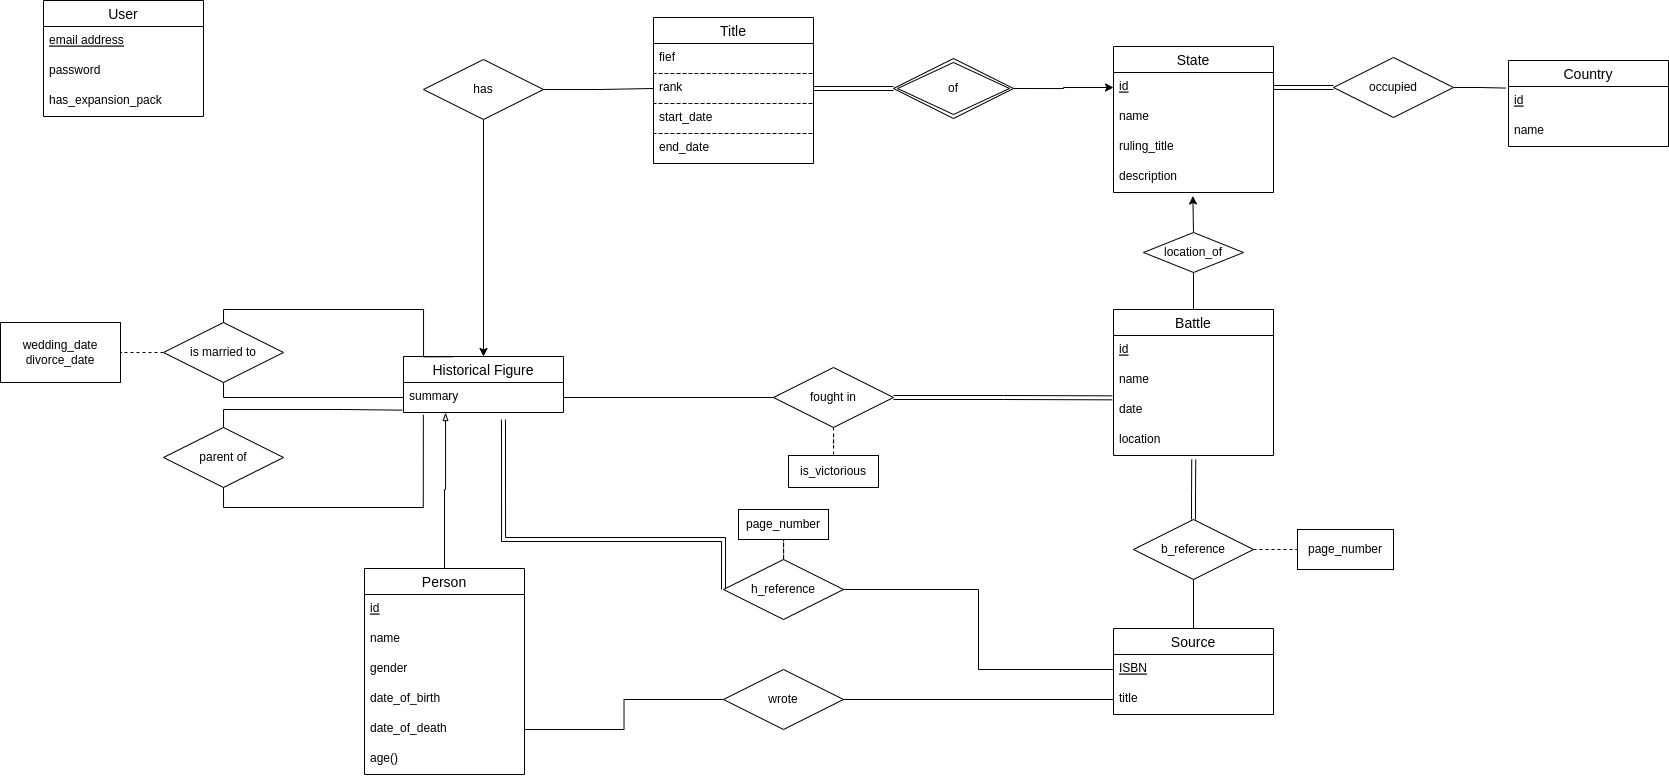
\includegraphics[width=.9\linewidth]{./er-diagram.drawio.png}
\end{center}
\section{Relational schema}
\label{sec:org2166e97}
\begin{itemize}
\item person ( \uline{id}: integer, name: string, gender: string, date\_of\_birth: date, date\_of\_death: date, age: integer )
\item historical\_figure ( \uline{id*}: integer, summary: string )
\item state ( \uline{id}: integer, name: string, description: string, ruling\_title: string )
\item country ( \uline{id}: integer, name: string )
\item battle ( \uline{id}: integer, name: string, date: date, location: (float, float), state\_id*: integer )
\item source ( \uline{ISBN}: string, title: string )
\item user ( \uline{email\_address}: string, password: string, has\_expansion\_pack: boolean )
\item title ( \uline{state\_id*}: integer , \uline{fief}: string, \uline{rank}: string, \uline{start\_date}: date, \uline{end\_date}: date, historical\_figure\_id*: integer )
\end{itemize}

\begin{itemize}
\item is\_married\_to ( \uline{person\_id*}: integer, \uline{person2\_id*}: integer, wedding\_date: date, divorce\_date: date )
\item parent\_of ( \uline{parent\_id*}: integer, \uline{child\_id*}: integer )
\item occupied ( \uline{state\_id*}: integer, \uline{country\_id*}: integer )
\item b\_reference ( \uline{battle\_id*}: integer, \uline{ISBN*}: string, page\_number: integer )
\item h\_reference ( \uline{historical\_figure\_id*}: integer, \uline{ISBN*}: string, page\_number: integer )
\item fought\_in ( \uline{historical\_figure\_id*}: integer, \uline{battle\_id*}: integer, is\_victorious: boolean )
\item wrote ( \uline{person\_id*}: integer, \uline{ISBN*}: string )
\end{itemize}

\section{Design}
\label{sec:orge9fcb07}
\subsection{ER Model}
\label{sec:org72b218d}
For the ER model I first identified nouns and then the attributes as follows.
\begin{itemize}
\item Person
\begin{itemize}
\item name, gender, date\_of\_birth, date\_of\_death, age()
\end{itemize}
\item Historical figure inherited from person
\begin{itemize}
\item summary
\end{itemize}
\item Title (weak set)
\begin{itemize}
\item fief, rank, duration
\end{itemize}
\item State
\begin{itemize}
\item name, description, ruling title
\end{itemize}
\item Modern country
\begin{itemize}
\item name
\end{itemize}
\item Battle
\begin{itemize}
\item name, date, location
\end{itemize}
\item Source
\begin{itemize}
\item title, ISBN
\end{itemize}
\item User
\begin{itemize}
\item email, password, has\_expansion\_pack
\end{itemize}
\end{itemize}

Then I figured the relationships they should have between them as follows.
\begin{itemize}
\item Person and Person (person is parent of person)
\item Person and Person (person is married to person)
\item Person and Title (person has titles)
\item Title and State (title are of a state)
\item State and Modern Country (state occupied countries)
\item Battle and Person and State (battle between persons in state)
\end{itemize}

A historical figure and a battle can only have a book as a reference for a single page. This constraint is added because of the specification. This can be changed by making the page number attribute of the relationship multi-valued.\\

A battle is fought in a single state or no state.\\

I used a superclass ``person'' for historical figure as it allows non-historic figures to be authors of sources as well.\\

Title is a weak entity set because there is candidate key and so that no information is lost.\\

The user entity can have bookmarks and other features depending on the scenario but this is enough for the base scenario.\\

Relationship attributes was neccessary because of many-to-many relationship and made the diagram consise and easy to understand.\\

The only derived attribute is the age of a person, and while it can be a simple attribute it makes more sense this way as the information needed to compute it is already available.\\

The battle name could be the primary key but that would require the assumption that each battle name is unique which might or might not be true.

\subsection{Relational Schema}
\label{sec:org0e8dcb0}
Here I simply transferred the attributes to the schema. In cases of one-to-many or many-to-one relations, I added a foreign key of the ``many'' entity set to the ``one'' entity set. In the case of many-to-many relations, I added relational schemas with private keys of both entity sets along with relation attributes where applicable.\\

I chose a tuple of two floats for the location to be specific.
\subsection{Normalisation}
\label{sec:org97820c9}
The full functional dependencies are as follows
\subsubsection{person}
\label{sec:org6a7289c}
id -> name\\
id -> gender\\
id -> date\_of\_birth\\
id -> date\_of\_death\\
id -> age\\
\{ date\_of\_birth, date\_of\_death \} -> age\\
\subsubsection{historical\_figure}
\label{sec:org6e4730e}
id -> summary\\
\subsubsection{state}
\label{sec:org0e6651c}
id -> name\\
id -> description\\
id -> ruling\_title\\
\subsubsection{country}
\label{sec:orgb9eb24a}
id -> name\\
\subsubsection{battle}
\label{sec:org19aa1bf}
id -> name\\
id -> date\\
id -> location\\
id -> state\_id\\
\subsubsection{source}
\label{sec:org8deaf9b}
ISBN -> title\\
\subsubsection{user}
\label{sec:orgc35d404}
email\_address -> password\\
email\_address -> has\_expansion\_pack\\
\subsubsection{title}
\label{sec:org92d182b}
\{ state\_id, fief, rank, start\_date, end\_date \} -> historical\_figure\_id\\

\subsubsection{Conclusion}
\label{sec:org6a1278b}
It is 1NF because there is no searching using a name given in the scenario and all relevant relational access is atomic.\\

It is 2NF because all non-prime attributes are fully functionally dependent on the candidate keys.\\

Not a 3NF or BCNF because a derived attribute exists. A derived attribute is a transitive dependency. In this case in the relation, person, there exists\\
id -> date\_of\_birth\\
id -> date\_of\_death\\
\{ date\_of\_birth, date\_of\_death \} -> age\\
id -> age\\

Thinking about it, the id in battle might be dependent on the attributes - name, date, location.

\section{Conclusion}
\label{sec:org24b39af}
This practical reinforced the theory learnt and helped practice building database models.
\end{document}
